\section{Optimal Control of Pitch/Travel with Feedback (LQ)}\label{sec:prob3}

\subsection{Discrete LQR}
\label{text:LQR}

To eliminate the discrepency between the optimal and measured trajectory observed in figure \ref{fig:opt_openloop}, we can update the optimal trajectory for every time step with a state feedback term weighted by a suitable gain matrix $K$:
\begin{equation*}
u_k = u_k^* - K^\top(x_k - x_k^*),
\end{equation*}

or, alternatively
\begin{equation}
\label{eq:LQ_ctrl}
\Delta u_k = - K^\top \Delta x_k,
\end{equation}

where 
\begin{align*}
\Delta x_k &= x_k - x_k^*,\\
\Delta u_k &= u_k - u_k^*.
\end{align*}

It can be shown (some clever reference here...) that the controller \eqref{eq:LQ_ctrl} is the optimal solution minimizing the quadratic objective function

\begin{equation*}
	J = \sum_{i=0}^{\infty} \Delta x_{i+1}^\top \tilde{Q} \Delta x_{i+1} + \Delta u_i^\top \tilde{R} \Delta u_i,
\end{equation*}

subject to the system dynamics \eqref{eq:dmodel}, where
\begin{equation}
\label{eq:LQ_gain}
	K = (R + B^\top P B)^{-1} B^\top P A,
\end{equation}

and $P$ is the unique positive definite solution to the discrete time algebraic Riccati equation.\eqref{eq:LQ_gain} is used as the state feedback gain, and the resulting Linear Quadratic controller is implemented, with weigthing matrices $Q$ and $R$ chosen to penalize deviations in states and input for a satisfactory results.

\subsection{Results and discussion}
Maybe discuss (L)QR (pun intended), tuning...
\begin{equation*}
\tilde{Q} = \begin{bmatrix}4&0&0&0\\0&2&0&0\\0&0&0&0\\0&0&0&0\end{bmatrix}, \quad \tilde{R} = 0.1.
\end{equation*}

Using MATLAB's \texttt{dlqr} we obtain the LQ state feedback gain, and the controller is applied with results shown in figure \ref{fig:lqr}.

\begin{figure}[hp]
	\centering
		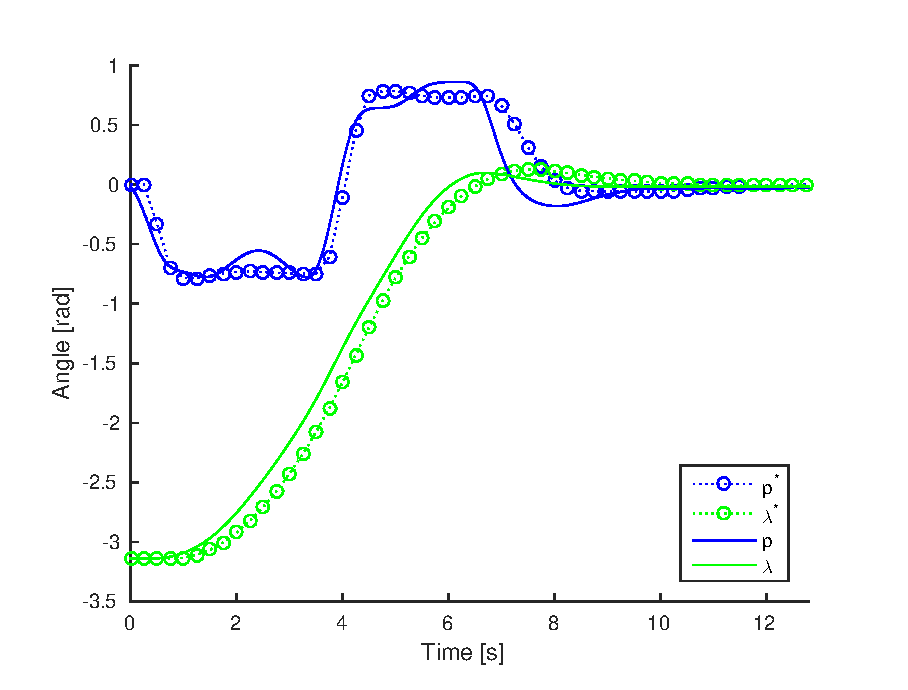
\includegraphics[width=0.85\textwidth]{figures/3/closedloop.eps}
	\caption{LQR}
	\label{fig:lqr}
\end{figure}

\subsubsection{MPC discussion}

